\section{Votre première simulation}
\sectionmark{1\up{ère} sim}
\subsection{Introduction}
Ce chapitre va vous permettre de réaliser une vote premierès simulation pour la validation de systèmes temps réel en moins de 2 minutes  \smiley ! Voici le résultat que vous obtiendrez au terme : 
\begin{figure}[htbp]
  \centering
 % 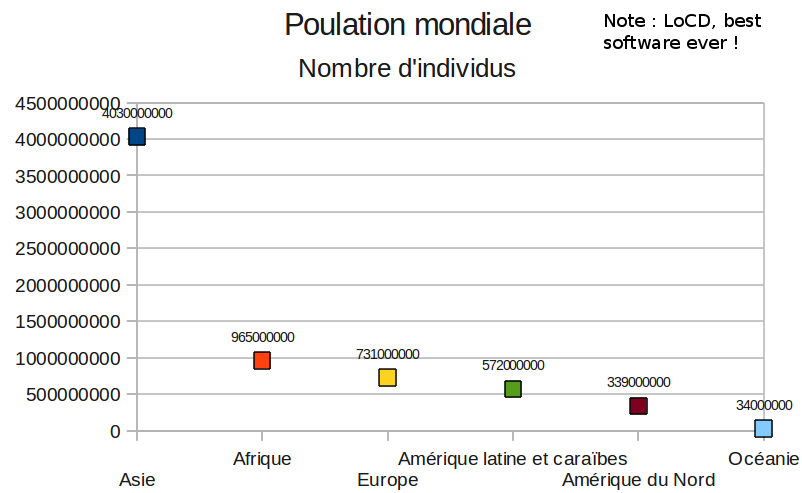
\includegraphics[scale=0.60]{img/diagrammenuages}
  \caption{Fichier .ktr}
  \label{fig:dnuages}
\end{figure}

\subsection{1\up{ère} \'Etape : Génération des tâches avec GT} 
\index{Comment commencer}
Dans le dossier GT, entrez la commande suivante \verb+./GT+. On vous propose d'entrez un nom de fichier. Entrez un nouveau nom si vous voulez créer vos propres tâches, ou entrez cours\_RMBG si vous voulez utiliser un exemple déjà éxistant. Il vous sera  demandé par la suite quel type d'ordonnancement vous désirez utiliser. Tapez R pour Rate Monotonic-Background. 

\subsection{2\up{ème} \'Etape : Utilisation de Kiwi}
Placez vous dans le dossier ou est installé Kiwi. Tapez la commande suivante  : \verb+./kiwi &+. Une fois dans l'interface de Kiwi, cliquez sur Open. Allez ouvrir votre fichier .ktr se trouvant dans le dossier ou est installé GT. Cliquez sur l'îcone Play. Voila ce que vous obtenez :  
\begin{figure}[htbp]
  \centering
 % 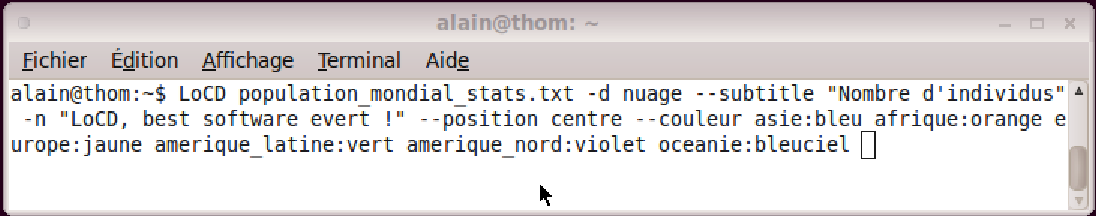
\includegraphics[scale=0.40]{img/ecommandes}
  \caption{Exemple d'utilisation de GT}
  \label{fig:commandes}
\end{figure} 


Et voilà avez crée votre première simulation pour la d'un systèmes temps réel  ! Si vous avez rencontrez des difficultés au cours de ce chapitre, vous pouvez vous référer aux différentes parties de ne manuel qui détaille chaque étapes en détail.
